\section{Bildverarbeitung}

\textbf{Ebenen von Computer Vision}:
\begin{itemize}
	\item \textbf{High-level Vision}: Objekterkennung
	\item \textbf{Mid-level Vision}: Segmentierung, Line Fitting
	\item \textbf{Low-level Vision}: Rauschunterdrückung, Kontrasterhöhung
\end{itemize}
\bigskip
\textbf{Monochrombild} (Graustufenbilder): Für jedes Pixel wird ein Helligkeitswert abgelegt: $\text{Img}\colon [0\cdots n-1]\times [0\cdots m-1]\rightarrow [0\cdots q]$, normalerweise ist $q=255$ also ein Byte\\

\textbf{Auflösung}: Gibt an, wie viel Pixel im Bild vorhanden sind\\

\textbf{RGB Farbraum}: Pixel wird durch 3 Bytes repräsentiert (rot, grün, blau):\\
$\text{Img}\colon [0\cdots n-1]\times [0\cdots m-1]\rightarrow [0\cdots R]\times[0\cdots G]\times [0\cdots B]$\\

\textbf{HSI Farbraum}: Speichert Hue (Farbton), Saturation (Sättigung), Intensity (Lichtintensität/Helligkeit). \textbf{Umrechnung RGB in HSI}:
\begin{center}
	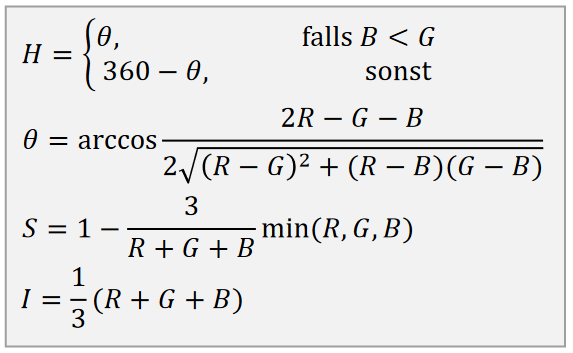
\includegraphics[width=0.4\textwidth]{images/hsi.png}
\end{center}

\textbf{Bildrepräsentation im Speicher}: Pixel werden zeilenweise abgelegt
\begin{center}
	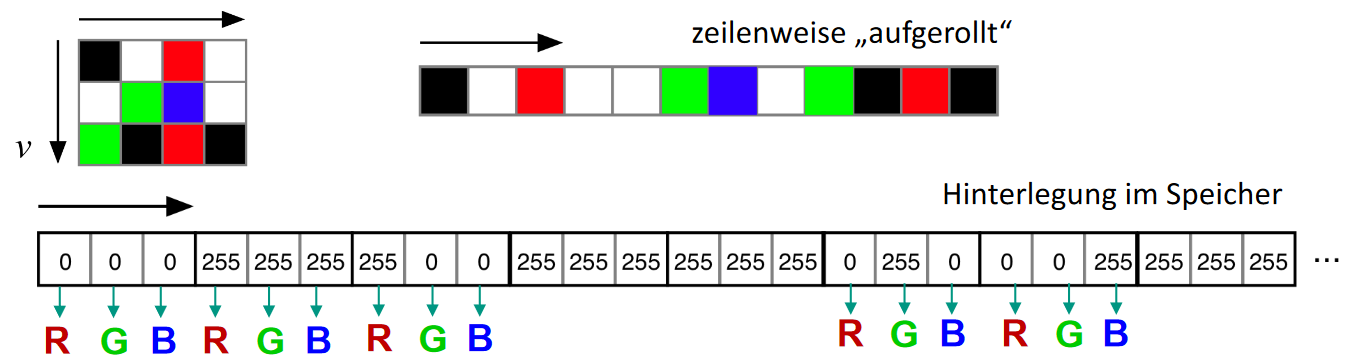
\includegraphics[width=0.7\textwidth]{images/repr.png}
\end{center}

\textbf{3D-Tiefenbilder}: Zusätzlich zur visuellen Information kann die Entfernung zum Sensor pro Pixel gespeichert werden: $\text{Img}(u,v)=(r,g,b,d)^\top$\\

\textbf{Punktwolken}:
\begin{itemize}
	\item Diskrete Menge von 3D-Punkten mit einem festen Koordinatensystem
	\item Punktwolke $P=\{(X,C)\mid X\in\R^3, C\in [0\ldots 255]^3\subset \N_0^3\}$, wobei $X=(x,y,z)$ Ortsinformation und $C = (r,g,b)$ Farbinformation
\end{itemize}
\bigskip
\textbf{Lochkamera-Modell}:
\begin{center}
	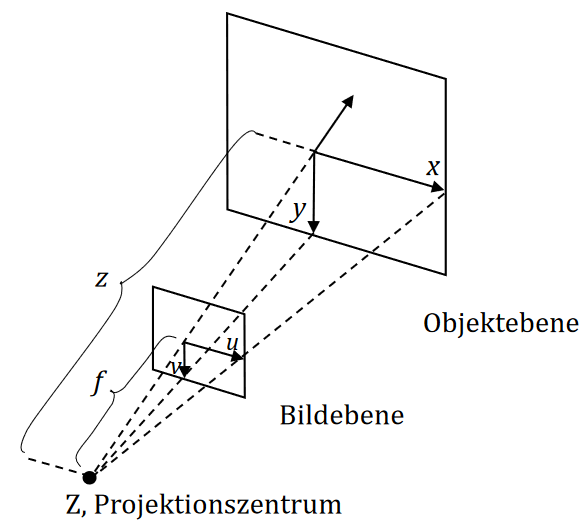
\includegraphics[width=0.4\textwidth]{images/lochkamera.png}
\end{center}
\begin{itemize}
	\item $f$ heißt \textbf{Brennweite}
	\item \textbf{Hauptachse}: Gerade durch das Projektionszentrum, rechtwinklig zur Bildebene
	\item \textbf{Hauptpunkt}: Schnitt der Hauptachse mit der Bildebene
	\item \textbf{Bildkoordinaten}: 2D-Koordinaten $(u,v)$ eines Punktes im Bild
	\item \textbf{Kamerakoordinatensystem}: 3D-Koordinaten $(x,y,z)$ eines Punktes relativ zur Kamera
	\item \textbf{Weltkoordinatensystem}: 3D-Basiskoordinatensystem in der Welt
	\item Mit Strahlensatz gilt:
	$$\left(
	\begin{matrix}
		u \\
		v
	\end{matrix}\right)=\frac{f}{z}\left(
	\begin{matrix}
	x \\
	y
	\end{matrix}\right)$$
	\item Wenn Sensor in der Lage ist Tiefenwerte $d$ für jedes Pixel zu bestimmen, dann gilt: $$\left(
	\begin{matrix}
		x \\
		y \\
		z
	\end{matrix}\right)=\frac{d}{f}\left(
	\begin{matrix}
		u \\
		v \\
		1
	\end{matrix}\right)$$
\end{itemize}
\bigskip
\textbf{Erweitertes Kameramodell}:
\begin{itemize}
	\item Unabhängige Brennweiten $f_x$ und $f_y$ in $u$ und $v$ Richtung, also $f=\left(
	\begin{matrix}
		f_x \\
		f_y
	\end{matrix}\right)$
	\pagebreak
	
	\item Es gilt:
	$$
	\left(\begin{array}{l}
		u \\
		v \\
		1
	\end{array}\right)=\left(\begin{array}{ccc}
		\frac{f_{x}}{z} & 0 & \frac{c_{x}}{z} \\
		0 & \frac{f_{y}}{z} & \frac{c_{y}}{z} \\
		0 & 0 & \frac{1}{z}
	\end{array}\right)\left(\begin{array}{l}
		x \\
		y \\
		z
	\end{array}\right) \Rightarrow\left(\begin{array}{c}
		u \cdot z \\
		v \cdot z \\
		z
	\end{array}\right)=\underbrace{\left(\begin{array}{ccc}
			f_{x} & 0 & c_{x} \\
			0 & f_{y} & c_{y} \\
			0 & 0 & 1
		\end{array}\right)}_{K}\left(\begin{array}{l}
		x \\
		y \\
		z
	\end{array}\right)
	$$
	wobei $K$ die \textbf{Kalibriermatrix} und $(c_x,c_y)$ der Hauptpunkt ist
	\item Parameter in Kalibriermatrix $K$ werden als \textbf{intrinsische Parameter} bezeichnet
	\item Beziehung zwischen Kamera-Koordinatensystem und Weltkoordinatensystem wird durch die \textbf{extrinsischen Parameter} beschrieben: eine Rotation $R$ und eine Translation $t$ im Raum
	\item Projektion eines Punktes von Weltkoordinaten auf Bildkoordinaten ist durch die \textbf{Projektionsmatrix} $P$ gegeben: $P=K\cdot(R\mid t)$
\end{itemize}
\bigskip
\textbf{Filteroperationen}:
\begin{itemize}
	\item Maskenwerte werden mit den darunter liegenden Pixelwerten multipliziert und das Ergebnis aufsummiert 
	\begin{center}
		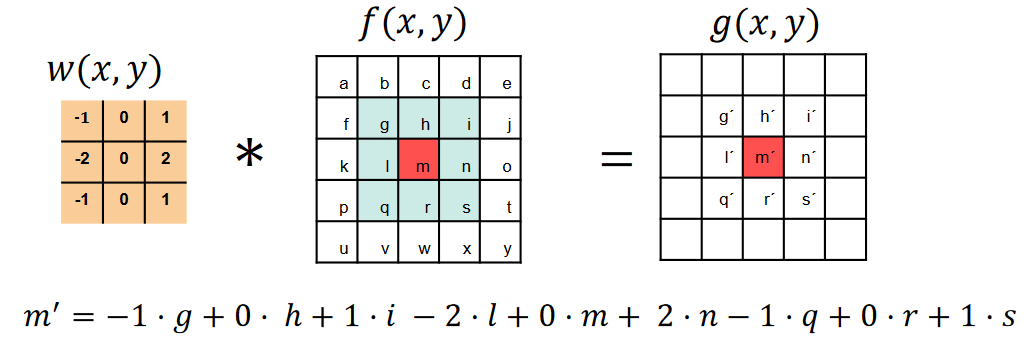
\includegraphics[width=0.6\textwidth]{images/filter.png}
	\end{center}
	\item Ränder werden häufig abgeschnitten, oder Ränder mit künstlichen Pixeln aufgefüllt (\textbf{Padding}):
	\begin{itemize}
		\item \textbf{Konstanter Wert}, z.B. Bild wird an den Rändern auf 0 gesetzt
		\item \textbf{Umschlingen}: Bild wird fortgesetzt
		\item \textbf{Spiegeln}: Bild wird an den Rändern gespiegelt
		\item \textbf{Wiederholen}: Nehme letzten Wert
	\end{itemize}
	\item Bei Farbbildern hat jedes Filter hat eine Filtermatrix (\textbf{Kernel}) pro Eingabekanal
\end{itemize}
\bigskip
Es folgen \textbf{Tiefpassfilter} zur Glättung und Rauschelimination.

\textbf{Mittelwertfilter}:
$$W_\text{Mittelwert}=\frac{1}{9}\left(
\begin{matrix}
	1 & 1 & 1 \\
	1 & 1 & 1 \\
	1 & 1 & 1 
\end{matrix}\right)$$
\pagebreak

\textbf{Medianfilter}:
\begin{center}
	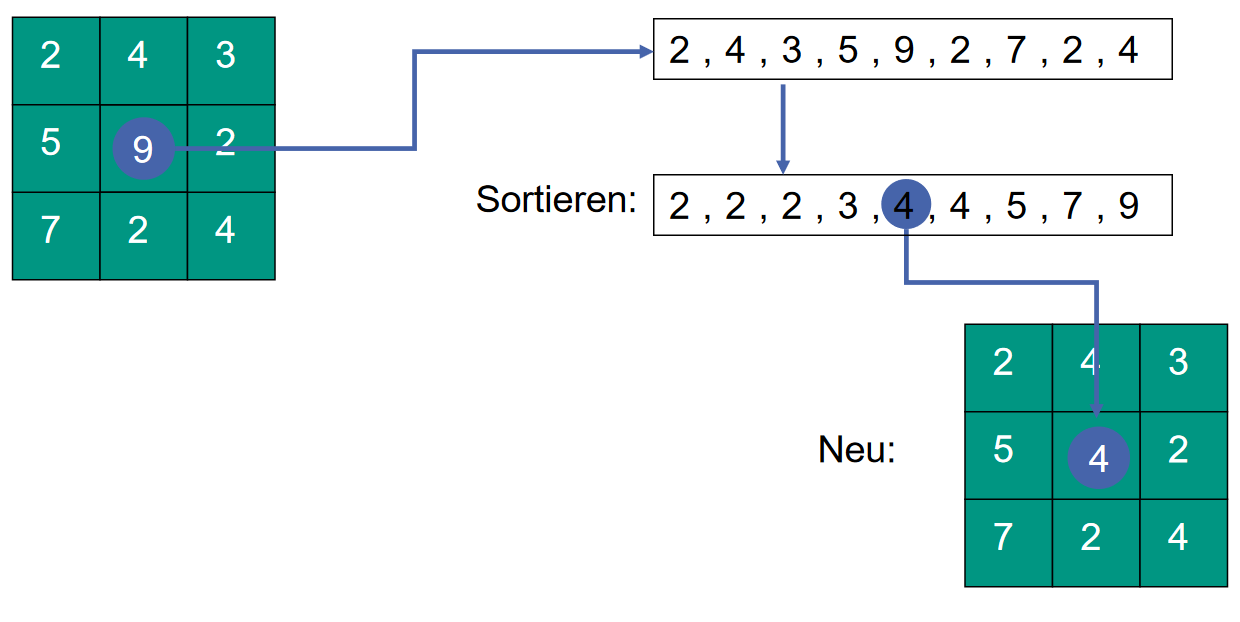
\includegraphics[width=0.6\textwidth]{images/median.png}
\end{center}

\textbf{Gauß-Filter}: Definiert durch zweidimensionale Gauß-Funktion
$$w(x,y)=\frac{1}{2\pi\sigma^2}e^{-\frac{x^2+y^2}{2\sigma^2}}$$

Es folgen \textbf{Hochpassfilter} zur Kantendetektion.
\textbf{Prewitt Filter}:
\begin{itemize}
	\item \textbf{Prewitt-X Filter}: $$p_x=\left(
	\begin{matrix}
		-1 & 0 & 1 \\
		-1 & 0 & 1 \\
		-1 & 0 & 1 
	\end{matrix}\right)$$
	\item \textbf{Prewitt-Y Filter}: $$p_y=\left(
	\begin{matrix}
		-1 & -1 & -1 \\
		0 & 0 & 0 \\
		1 & 1 & 1 
	\end{matrix}\right)$$
	\item Gute Ergebnisse bei Detektion von vertikalen bzw. horizontalen Kanten
\end{itemize}

\textbf{Sobel Filter}:
\begin{itemize}
	\item \textbf{Sobel-X Filter}: $$s_x=\left(
	\begin{matrix}
		-1 & 0 & 1 \\
		-2 & 0 & 2 \\
		-1 & 0 & 1 
	\end{matrix}\right)$$
	\item \textbf{Sobel-Y Filter}: $$s_y=\left(
	\begin{matrix}
		-1 & -2 & -1 \\
		0 & 0 & 0 \\
		1 & 2 & 1 
	\end{matrix}\right)$$
	\item Ähnlich wie Prewitt, gewichtet aber das Zentrum des betrachteten Fensters stärker
\end{itemize}

\textbf{Weitere Filter}, s. \textit{9/88-94}\\
\pagebreak

\textbf{Morphologische Operatoren}:
\begin{itemize}
	\item \textbf{Dilatation}: Alle Werte der Ergebnismatrix zu 0 setzen. Ein Wert der Ergebnismatrix wird zu $q$, wenn $q$ min. an einer Stelle im $3\times 3$-Block vorkommt
	\item \textbf{Erosion}: Alle Werte der Ergebnismatrix zu 0 setzen. Ein Wert der Ergebnismatrix wird zu $q$, wenn $q$ an allen Stellen im $3\times 3$-Block vorkommt
	\item \textbf{Öffnen}: Anwendung von Erosion danach Dilatation, Entfernt dünne Linien oder kleine außenliegende Bereiche
	\item \textbf{Schließen}: Anwendung von Dilatation danach Erosion, Überbrückung kleiner Distanzen und Schließung von inneren Löchern
\end{itemize}
\bigskip
\textbf{Segmentierung}: Aufteilung einer Menge in aussagekräftige Segmente

\textbf{Schwellenwertfilterung}: Intensität von jedem Pixel $(u,v)$ wird mit einem vordefinierten Schwellwert $T$ verglichen
$$\text{Img'}(u,v)=\begin{cases}
	255\;, & \text{falls Img}(u,v)>T\\
	0\;, & \text{sonst}
\end{cases}$$
\begin{itemize}
	\item Objekte können auch über ihre Farbe segmentiert werden $\rightarrow$ Vergleiche z.B. $H,S,I$ Werte
	\item \textbf{Problem}: Wechselnde Lichtbedingungen, Reflexionen, Schattenwürfe
\end{itemize}
\bigskip
\textbf{Canny-Kantendetektor}:
\begin{itemize}
	\item Basiert auf 3 Grundsätzen:
	\begin{enumerate}
		\item \textbf{Geringe Fehlerrate}: Alle Kanten sollen gefunden werden und detektierte Kanten sollten so nah wie möglich an den realen Kanten sein
		\item \textbf{Gute Detektion}: Distanz zwischen detektierten Kantenpunkten und dem Zentrum der realen Kanten soll minimal sein
		\item \textbf{Eindeutigkeit}: Detektor liefert nur ein Punkt zu einem realen Kantenpunkt
	\end{enumerate}
	\item \textbf{Algorithmus}:
	\begin{enumerate}
		\item \textbf{Gauß-Filter} $\rightarrow$ Rauschunterdrückung
		\item Berechnung der \textbf{Intensitätsgradienten}
		\item \textbf{Non-Maximum Suppression}: Kantenausdünnung. Alle Pixel, die kein Maximum darstellen, werden unterdrückt
		\item \textbf{Double Threshold} zur Entfernung schwach verbundener Kantenpixel
		\item Kantenverfolgung mit \textbf{Hysterese}
	\end{enumerate}
\end{itemize}

\textbf{Visual Servoing}: Verfahren bei denen visuelle Eingabedaten genutzt werden, um die Bewegung eines Roboters zu steuern
\begin{itemize}
	\item \textbf{Kamera-in-Hand} oder \textbf{externe (feste) Kamera}
	\item \textbf{Interaction Matrix / Image Jacobian} beschreibt die Beziehung zwischen der Geschwindigkeiten eines Bildmerkmals und eines der Kamera:
	$$\dot{s}=L(u,v,z)\cdot\dot{p}$$
\end{itemize}
\bigskip
\textbf{Registrierung von Punktwolken}: Zusammenführen von Punktwolken, welche das gleiche Objekt aus unterschiedlichen Ansichten beschreibt

\textbf{Iterative Closest Point}: Algorithmus für die Registrierung zweier Mengen $A,B$
\begin{itemize}
	\item Durchführung siehe Übungsblatt 7
	\item \textbf{Vorteile}: Algorithmus für viele Darstellungsformen anwendbar, Einfache mathematische Operationen, Schnelles Registrierungsergebnis
	\item \textbf{Nachteile}: Überlappung der Punktwolken erforderlich, Symmetrische Objekte können nicht registriert werden, Konvergenz in ein lokales Minimum möglich
\end{itemize}
\bigskip
\textbf{RANSAC - Random Sample Consensus}:
\begin{itemize}
	\item Iterative Methode zur Schätzung von Modellparametern aus Datenpunkten
	\item \textbf{Algorithmus}:
	\begin{enumerate}
		\item Wähle zufällig die minimale Anzahl an Punkten aus, die nötig ist um die Modellparameter zu berechnen
		\item Schätzung des Modell aus dem ausgewählten Datensatz
		\item Bewertung der Modellschätzung
		\item Wiederhole 1-3 bis das Modell mit den meisten Inliers gefunden wird
	\end{enumerate}
	\item \textbf{Vorteile}: Einfach zu implementieren, Robuste Modellschätzung für Daten mit wenigen Ausreißern, Vielseitig anwendbar
	\item \textbf{Nachteile}: Nicht-deterministisch, Benötigt viele Iterationen, Nicht anwendbar wenn das Verhältnis Inliers/Outliers zu klein ist
\end{itemize}
\pagebreak